\documentclass{article}
\usepackage{graphicx} % Required for inserting images
\usepackage[backend=biber]{biblatex}
\usepackage{hyperref}
\hypersetup{
    colorlinks=true,
    linkcolor=blue,
    filecolor=magenta,      
    urlcolor=cyan,
    pdftitle={Overleaf Example},
    pdfpagemode=FullScreen,
    }

\addbibresource{bibliography.bib}

\title{Machine Learning For Data Science I, \\[0.1cm] Homework 04}

\author{Maj Gaberšček, 27212075}
\date{April 2023}

\begin{document}

\maketitle

\section*{Problem}

The problem of this homework consisted of firstly implementing the multinomial logistic regression model and ordinal regression model. Both models should be implemented as classes and also have methods to build them and predict on new samples.

Secondly, we applied multinomial logistic regression on basketball dataset and had to interpret results. Lastly, we had to implement a data generating process, where multinomial logistic regression would perform worse then the ordinal regression.

\section{Part I: models}

Both models are implemented as each class in the Python code. Every method of each class is well described and documented within the code, so I will not be describing it again in this report.

\section{Part II: interpretation}

In this part of the homework, we had to apply multinomial logistic regression model to basketball database. Firstly, the \texttt{dataset.csv} file contains data from over 5024 basketball shots in real-world basketball games. Our task was to firstly preprocess the dataset, so that it fits our multinomial regression model. Preprocessing took place in code function \texttt{data\_preparation}.

There is, a very detailed description of different mappings for different columns and also the reasoning behind those mappings in the code. It is necessary to emphasize, that I only used my basketball knowledge with the help of internet to make mappings. I could also check, how different values result in target variable and map values accordingly (to fit linear regression). However, then the model would be very prone to overfitting. So, after consideration, I decided not to take that approach.

For example, I mapped the movement column as (no: 1, dribble or cut: 3, drive: 4), as dribble or cut is more similar to drive as to no movement at all. Before applying the multinomial regression, I also normalized the data, to improve optimization convergence. I chose 'above head' to be the reference category. 

\subsection{Coefficients}

The coefficients are in the below table (they are rounded to 1 digit for better readability, even though confidence interval suggests different rounding for different coefficients):

\begin{table}[!ht]
    \centering
    \begin{tabular}{|l|l|l|l|l|l|l|l|l|}
    \hline
        class & comp. & player & trans. & two-l. & mov. & ang. & dist. & int. \\ \hline
        \textbf{above head} & 0.0 & 0.0 & 0.0 & 0.0 & 0.0 & 0.0 & 0.0 & 0.0 \\ \hline
        \textbf{layup} & -0.1 & 0.0 & 0.2 & 1.3 & 2.0 & 0.3 & -4.8 & -4.6 \\ \hline
        \textbf{other} & -0.2 & 0.1 & 0.0 & -0.3 & 0.9 & 0.0 & -0.4 & -2.0 \\ \hline
        \textbf{hook shot} & 0.3 & -0.2 & -0.2 & 0.2 & -1.7 & -0.2 & -2.2 & -3.4 \\ \hline
        \textbf{dunk} & 0.9 & -0.4 & 0.4 & 1.6 & -0.1 & -0.0 & -3.6 & -6.4 \\ \hline
        \textbf{tip-in} & 0.5 & -0.1 & 0.3 & 1.4 & -0.2 & -0.2 & -3.4 & -6.1 \\ \hline
    \end{tabular}
\end{table}

We have to of course look at the mappings to see the meaning of this coefficients. Some of the most obvious observations are:
\begin{itemize}
    \item Movement parameter strongly contributes towards shot being a layup (if movement is true) and against it being a hook shot. This makes sense, as almost all layups involve player movement while hook shots almost never do.
    \item With higher distance, probability of layup, dunk or tip-in drastically decreases. This also makes sense as all of this shots are almost always made from a very small distance. 
    \item An interesting remark is about the competition. As we mapped NBA to the highest number, high competition value contributes probability to dunk (as we almost never see dunks in youth selections and rarely in European basketball).
    \item Transition suggests higher probability for dunk, layup or tip-in, which again makes sense.
\end{itemize}

In the end I also calculated confidence interval for coefficients (by doing the bootstrapped confidence intervals). However, running several model-buildings for large datasets takes a lot of time (\texttt{fmin\_l\_bfgs\_b} needs quite a while to optimize). That is why I couldn't afford to sample with replacement a very large dataset. So I only built the model for 2000 random samples with replacement and did that 200 times. As I built with only 2000 samples, real confidence intervals (had I built with 5000 samples) are even more bounding than the ones in the table below.

Confidence intervals:

\begin{table}[!ht]
\centering
\begin{tabular}{|l|l|l|l|l|}
\hline
class & competition & player type & transition & two-legged \\ \hline
\textbf{above head} & (0.0, 0.0) & (0.0, 0.0) & (0.0, 0.0) & (0.0, 0.0) \\ \hline
\textbf{layup} & (-0.29, 0.17) & (-0.12, 0.24) & (-0.02, 0.4) & (0.91, 1.68) \\ \hline
\textbf{other} & (-0.47, -0.01) & (-0.07, 0.31) & (-0.23, 0.18) & (-0.7, 0.12) \\ \hline
\textbf{hook shot} & (0.07, 0.43) & (-0.39, -0.01) & (-0.54, 0.1) & (-0.09, 0.49) \\ \hline
\textbf{dunk} & (0.59, 1.3) & (-0.85, -0.07) & (-0.05, 0.69) & (0.91, 2.01) \\ \hline
\textbf{tip-in} & (0.22, 0.91) & (-0.6, 0.3) & (-0.28, 0.64) & (0.64, 1.83) \\ \hline
\end{tabular}
\end{table}

\begin{table}[!ht]
\centering
\begin{tabular}{|l|l|l|l|l|}
\hline
class & movement & angle & distance & intercept \\ \hline
\textbf{above head} & (0.0, 0.0) & (0.0, 0.0) & (0.0, 0.0) & (0.0, 0.0) \\ \hline
\textbf{layup} & (1.66, 2.43) & (0.05, 0.49) & (-5.63, -3.93) & (-5.34, -3.65) \\ \hline
\textbf{other} & (0.6, 1.32) & (-0.16, 0.21) & (-0.7, 0.01) & (-2.29, -1.82) \\ \hline
\textbf{hook shot} & (-2.07, -0.87) & (-0.4, 0.0) & (-2.52, -1.93) & (-3.79, -3.18) \\ \hline
\textbf{dunk} & (-0.38, 0.18) & (-0.37, 0.36) & (-4.22, -2.65) & (-7.09, -5.28) \\ \hline
\textbf{tip-in} & (-0.45, 0.11) & (-0.54, 0.21) & (-4.0, -2.32) & (-6.72, -5.16) \\ \hline
\end{tabular}
\end{table}

\section{Part III: the DGP}

Here, we had to define a data-generating process, for which the ordinal regression model would perform better then the multinomial regression.

My process describes football games and has 4 attributes: earned points of home and away team in their last game and strength of home and away team (strong or weak). The target variable is outcome of the game for the home team (win, draw or loss).

First I check the point difference (first and second attribute) and then define probabilities of outcome. Then the probabilites are tweaked by difference in team strength. Then I return target value randomly (probabilities are weights).

Naturally, ordinal regression should perform better, as classes are ordered (loss; draw; win). I built both models on 1000 samples and then tested them on 1000 other samples. As expected, log-likelihood was bigger (model was better) for ordinal logistic regression (-911.7), as compared to multinomial logistic regression (-917.2).

\section{Other information}
The report is of course only 2 pages, so some things had to be left out. That is why the code is nicely documented and there are several comments to explain it. If you are interested in code history (past bugs, that have been solved, etc.), also feel free to visit this courses's homework \href{https://github.com/majbc1999/ml-for-data-science-homeworks} {Github repository}.

% FIGURE EXAMPLE
%\begin{figure}[!h]
%    \centering
%    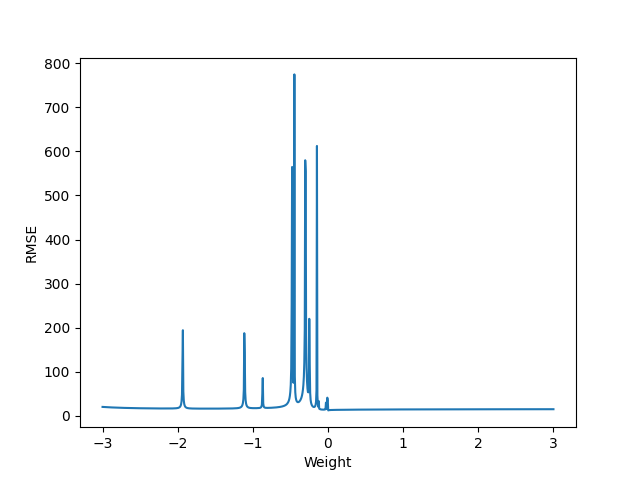
\includegraphics[width=0.7\textwidth]{homework-03/plots/ridge.png}
%    \caption{RMSE for different $\lambda$ (weight) of L2 regression}
%    \label{fig:f}
%\end{figure}


\printbibliography

\end{document}